
\label{sect:data}

We collect a set of galaxy spectroscopic redshifts, paired with broadband photometry, from various surveys to test our training algorithm.
Our set consists of 102,476 galaxies with redshifts $z < 4.54$ and $i$-band magnitudes\footnote{The $i$-band magnitudes quoted in this section denote the magnitude in one of $i$, $i_2$, $I$, or $i^+$ as listed in Table \ref{tab:filters}. For galaxies with photometry in multiple $i$-bands, the magnitude used is the first to appear in that list.} in the range $13.8 < i < 25.7$.
For all surveys, we use galaxies with highly reliable spec-z's, photometry in one of the $i$-bands, and photometry in at least three bands with signal-to-noise ratio SNR $> 20$.
The entire data set is summarized in Table \ref{tab:data_sets}, the filters used to measure the photometry are listed in Table \ref{tab:filters}, and the redshift distributions are shown in Figure \ref{fig:redshift_dist}.

\begin{table*}
    \caption{Summary of the spec-z and photometry data sets. $N_\text{gal}$ is the total number of galaxies in the set, $f_\text{gal}$ is the fraction of galaxies in the set, and $\Bar{\sigma}_i$ is the mean fractional flux error for the $i$-band photometry.}
    \label{tab:data_sets}
    \centering
    \begin{tabular}{l r c c c c c c l}
        \toprule \toprule
        Data Set & $N_\text{gal}$ & $f_\text{gal}$ & $z_\text{mean}$ & $z_\text{max}$ & $i$-band range & $i_\text{mean}$ & $\Bar{\sigma}_i$ & Link to Catalog \\
        \midrule
        
        zCOSMOS  &  14298 & 0.14 & 0.57 & 2.52 & $16.87 \leq i \leq 24.18$ & 21.19 & 0.022 & \url{http://cesam.lam.fr/hstcosmos/} \\
        VVDS     &   6915 & 0.07 & 0.67 & 4.54 & $13.84 \leq i \leq 24.97$ & 20.86 & 0.014 & \url{https://cesam.lam.fr/vvds/index.php} \\
        VIPERS   &  69415 & 0.68 & 0.70 & 2.15 & $17.66 \leq i \leq 23.08$ & 21.38 & 0.017 & \url{http://vipers.inaf.it:8080/} \\
        DEEP2/3  &  10695 & 0.10 & 0.71 & 1.91 & $15.30 \leq i \leq 25.36$ & 21.42 & 0.020 & \url{http://d-scholarship.pitt.edu/36064/} \\
        3D-HST   &   1153 & 0.01 & 1.46 & 3.32 & $19.10 \leq i \leq 25.74$ & 23.56 & 0.027 & \url{http://d-scholarship.pitt.edu/36064/} \\
        \midrule
        Training &  81980 & 0.80 & 0.69 & 4.54 & $13.84 \leq i \leq 25.74$ & 21.32 & 0.018 & \\
        Test     &  20496 & 0.20 & 0.69 & 3.61 & $16.46 \leq i \leq 25.69$ & 21.34 & 0.018 & \\
        \midrule
        Total    & 102476 & 1.00 & 0.69 & 4.54 & $13.84 \leq i \leq 25.74$ & 21.33 & 0.018 & \\
        
        \bottomrule
    \end{tabular}
\end{table*}

\begin{table}
    \centering
    \caption{The 19 filters used to measure the galaxy photometry in the data set. Mean wavelength, $\lambda_0 = \int \lambda R(\lambda) d\lambda$, and effective width, $W_\text{eff} = \text{Max}[R(\lambda)]^{-1}$, are given in angstroms. Filters are listed in order of increasing $\lambda_0$. The system response functions for each filter were obtained from the Spanish Virtual Observatory (SVO) Filter Profile Service.}
    \begin{tabular}{l c c r r}
        \toprule \toprule
        Filter & Telescope & Instrument & $\lambda_0$ & $W_\text{eff}$ \\
        \midrule
        
        $NUV$ & GALEX  &         &  2343.1 &  767.3 \\
        $u$   & CFHT   & Megacam &  3817.7 &  525.4 \\
        $B$   & CFHT   & CFH12k  &  4342.5 &  873.6 \\
        $B_J$ & Subaru & Suprime &  4478.4 &  763.9 \\
        $g^+$ & Subaru & Suprime &  4808.5 & 1043.1 \\
        $g$   & CHFT   & Megacam &  4899.9 & 1293.8 \\
        $V$   & CFHT   & CFH12k  &  5393.7 &  882.7 \\
        $V_J$ & Subaru & Suprime &  5493.0 &  862.4 \\
        $r$   & CHFT   & Megacam &  6278.2 & 1120.2 \\
        $r^+$ & Subaru & Suprime &  6314.8 & 1211.4 \\
        $R$   & CFHT   & CFH12k  &  6603.5 & 1138.5 \\
        $i_2$ & CHFT   & Megacam &  7584.5 & 1409.4 \\
        $i$   & CHFT   & Megacam &  7676.6 & 1307.6 \\
        $i^+$ & Subaru & Suprime &  7709.1 & 1361.7 \\
        $I$   & CFHT   & CFH12k  &  8277.3 & 1816.7 \\
        $z$   & CHFT   & Megacam &  8857.6 & 1040.1 \\
        $z^+$ & Subaru & Suprime &  9054.5 & 1012.3 \\
        $Y$   & Subaru & Suprime & 10216.0 &  996.2 \\
        $J$   & UKIRT  & WFCAM   & 12508.5 & 1476.8 \\
        
        \bottomrule
    \end{tabular}
    \label{tab:filters}
\end{table}

\subsection{zCOSMOS-\textit{bright}}

zCOSMOS \citep{Lilly2009a} is a redshift survey of 1.7 $\text{deg}^2$ of the COSMOS field, conducted with the VIMOS spectrograph mounted on the European Southern Observatory's (ESO) Very Large Telescope (VLT).
The survey is divided into two parts, \textit{bright} and \textit{deep}. 
We make use of the former, consisting of approximately 20,000 galaxies with redshifts $z < 1.2$.
We use galaxies recommended in the ESO data release description\footnote{\url{https://www.eso.org/sci/observing/phase3/data_releases/zcosmos_dr3_b2.pdf}}, determined to have $99\%$ spectroscopic verification (i.e. \texttt{zflag} = 3.x, 4.x, 2.5, 2.4, 1.5, 9.5, 9.3, 18.5, 18.3).

The zCOSMOS redshifts are matched to photometry from \citet{Ilbert2009}.
The photometry is measured from the ultraviolent to the near-infrared in 11 broadband filters: $NUV$ on GALEX \citep{Martin2005a}, $u$ and $i$ on CFHT-Megacam, $B$ and $V$ on CFHT-CFH12k, $g^+$, $r^+$, $i^+$, and $z^+$ on Subaru, and $J$ on UKIRT.
The final set consists of 14,298 galaxies with redshifts $z < 2.52$ and $i$-band magnitudes in the range $16.9 < i < 24.2$.

\subsection{VVDS}

The VIMOS VLT Deep Survey (VVDS, \citealt{LeFevre2013b}) is a redshift survey consisting of three component surveys: \textit{Wide}, \textit{Deep}, and \textit{Ultra-Deep}. 
The Wide survey covers 8.7 $\text{deg}^2$, with approximately 25,000 galaxies in the range $17.5 < i < 22.5$; the Deep survey covers 0.74 $\text{deg}^2$, with approximately 11,000 galaxies in the range $17.5 < i < 24$; the Ultra-Deep survey covers 512 $\text{arcmin}^2$, with approximately 900 galaxies in the range $23 < i < 24.75$.
We use redshifts with quality flags 3 and 4, indicating a 98\% spec-z confidence.
The photometry was measured in nine filters: $u,g,r,i,z$ on CFHT-Megacam \citep{Hudelot2012} and $B,V,R,I$ on CFHT-CFH12k \citep{LeFevre2004}.
The final set contains 6,915 galaxies out to redshifts $z < 4.5$, with magnitudes $ 13.8 < i < 25.0$.

\subsection{VIPERS}

The VIMOS Public Extragalactic Redshift Survey (VIPERS, \citealt{Scodeggio2018a}) is a dense, large-volume redshift survey focusing on redshifts $0.5 < z < 1.2$.
We use VIPERS galaxies with spec-z's reliable at the 95\% confidence level (\texttt{zflag} = 2.X, 3.X, 4.X), and with \texttt{photoMask} and \texttt{spectroMask} = 1.
The redshifts are matched to photometry measured in $NUV$ on GALEX \citep{Martin2005a}, and $u,g,r,i_2,i,z$ on CFHT-Megacam\textsuperscript{\ref{ft:i2}} \citep{Hudelot2012}. 
The final set contains 71,951 galaxies with redshifts $z < 2.15$ and magnitudes $17.7 < i < 23.3$. 

\subsection{DEEP2 and DEEP3}

DEEP2 and DEEP3 are redshift surveys conducted with the DEIMOS spectrograph on the Keck 2 telescope.
DEEP2 \citep{Newman2013b} consists of four fields; we use galaxies from the first field in the Extended Groth Strip (EGS), which had no redshift pre-selection.
DEEP3 \citep{Cooper2011} expanded on the DEEP2 survey of the EGS.
Redshifts from these surveys are matched with aperture-corrected photometry provided by \citet{Zhou2019a}.
We use galaxies with CFHTLS flag 0, SExtractor flags less than 4 in every band, and redshift quality flag $\geq 3$.
Photometry was measured in $u,g,r,i_2,i,z$ on CFHT-Megacam\footnote{The $i_2$ band is the replacement to the Megacam $i$-band installed in 2007. This filter is named $y$ in the CFHTLS catalogues \citep{Hudelot2012}, but we follow \citet{Zhou2019a} in naming it $i_2$ to avoid confusion with the longer $y$ bands used in Subaru and LSST. \label{ft:i2}} and $Y$ on Subaru \citep{Miyazaki2002}.
The final set contains 10,695 galaxies with redshifts $z < 1.91$ and magnitudes $15.3 < i < 25.74$.


\subsection{3D-HST}

In addition to the spectroscopic surveys above, we include grism redshifts from the 3D-HST survey \citep{Newman2013b,Momcheva2016b}.
Redshifts for this survey were analyzed and matched with aperature-corrected photometry by \citet{Zhou2019a}.
We select the galaxies with CFHTLS flag 0, SExtractor flags less than 4 in every band, and the flag \texttt{use\_zgrism1} = 1.
For galaxies in both the DEEP2/3 and 3D-HST sets, we use DEEP2/3 redshifts instead.
Photometry was measured in $u,g,r,i_2,i,z$ on CFHT-Megacam and $Y$ on Subaru.
After these cuts, the 3D-HST set contains 1,153 galaxies with redshifts $z < 3.32$ and magnitudes $23.6 < i < 25.7$.

\begin{figure}
    \centering
    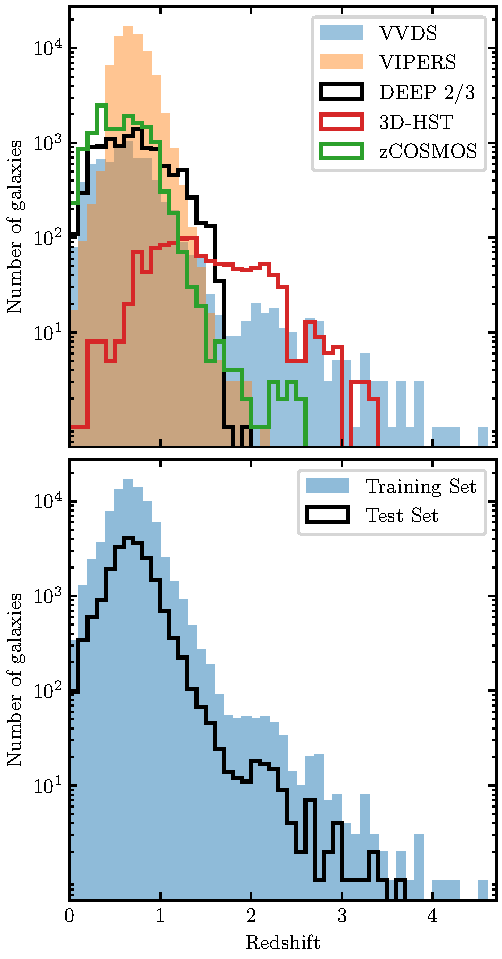
\includegraphics{figures/redshift_distribution.pdf}
    \caption{Redshift distribution of the galaxy surveys. The top panel shows the distributions of each of the constituent surveys. The bottom panel shows the redshift distributions of the training and test sets used for template training and photo-z estimation respectively.}
    \label{fig:redshift_dist}
\end{figure}

